\documentclass[journal=jprobs,manuscript=article]{achemso}
\usepackage[utf8]{inputenc}
\usepackage{amsmath}
\usepackage{hyperref}
\usepackage{fancyhdr}
\usepackage{graphicx}
\pagestyle{fancy}
\fancyhf{}
\cfoot{S-\thepage}

%\usepackage{changepage}   % For adjusting image width
%\usepackage{xr}

\fancypagestyle{firststyle}
{
   \fancyhead[R]{}
   \fancyhead[L]{}
   \fancyfoot[C]{}
}

\fancyfoot[C]{S-\thepage}
\fancyhead[R]{\textit{\small{Mouse primary T cell phosphoyrosine proteomics enabled by BOOST}}}
%\fancyhead[L]{\small{Chua \& Callahan \textit{et al.}}}
\fancyhead[L]{\small{Chua \textit{et al.}}}
\renewcommand{\figurename}{Supporting Figure}   % Renaming the Figure float name to "Supplementary Figure"
\renewcommand{\tablename}{Supporting Table}     % Renaming the Table float name to "Supplementary Table"

%%%%%%%%%%%%%%%%%%%%%%%%%%%%%%%%%%%%%%%%%%%%%%%%%%%%%%%%%%%%%%%%%%%%%%%%%%%%
% Originally, this was used to create a \beginsupplement command that would
% renumber and rename the figures and tables like above, however I removed
% this when I made the supplements their own document.
%\newcommand{\beginsupplement}{%
%            \setcounter{table}{0}
%            \renewcommand{\thetable}{Supplementary Table \arabic{table}}%
%            \setcounter{figure}{0}
%            \renewcommand{\thefigure}{\arabic{figure}}%
%     }
%%%%%%%%%%%%%%%%%%%%%%%%%%%%%%%%%%%%%%%%%%%%%%%%%%%%%%%%%%%%%%%%%%%%%%%%%%%%
\title{Supporting Information:  \\Mouse primary T cell phosphoyrosine proteomics enabled by BOOST}
\author{Xien Yu Chua$^{1}$, Kenneth P. Callahan$^{2}$, Alijah A. Griffith$^{2}$, Tobias Hildebrandt$^{2}$, Guoping Fu$^{3}$, Mengzhou Hu$^{1}$, Renren Wen$^{3}$, Arthur R. Salomon$^{2,*}$
\\
\singlespacing
\textit{\small{$1$ Department of Molecular Pharmacology, Physiology \& Biotechnology, Brown University, Providence, RI, 02912}}
\\
\textit{\small{$2$ Department of Molecular Biology, Cell Biology \& Biochemistry, Brown University, Providence, RI, 02912}}
\\
\textit{\small{$3$ Blood Research Institute, Blood Center of Wisconsin, Milwaukee, WI, 53226}}
\\
\textit{\small{$*$} Corresponding Author}\tiny}
\email{art@drsalomon.com}
%\\
%\textit{\small{$\P$ Contributed equally to this work}}\tiny}

%\author{Alijah A. Griffith}
%\altaffiliation{Contributed equally to this work}
%\author{Kenneth P. Callahan}
%\altaffiliation{Contributed equally to this work}
%\author{Nathan Gordo King}
%\affiliation[Brown University]{Department of Molecular Biology, Cell Biology \& Biochemistry, Brown University}
%\author{Qian Xiao}
%\author{Xiaolei Su} 
%\affiliation[Yale University]{Department of Cell Biology, Yale School of Medicine, Yale University}
%\author{Arthur R. Salomon}
%\email{art@drsalomon.com}
%\affiliation[Brown University]{Department of Molecular Biology, Cell Biology \& Biochemistry, Brown University}

%\date{September 2021}

\begin{document}
\pagenumbering{gobble}
\thispagestyle{firststyle}
\newpage
\begin{center}
\textbf{\underline{\large{Table Of Contents}}}
\end{center}

%\begin{table}[h!]
%    \begin{tabular}{ll}
%        \textbf{\hyperref[silaclabelingtable]{Supplementary Table} \ref{silaclabelingtable}:} & (.XLSX) Complete list of peptides identified after heavy   \\
%         & isotope labeling of Raji B cells and their labeling status. \\
%
 %       \textbf{\hyperref[ssh2totaltable]{Supplementary Table} \ref{ssh2totaltable}:} & (.XLSX) All peptides identified from sSH2 pTyr enrichment  \\
 %        & after coculture of CD19-CAR T cells and Raji B cells. \\
%
%        \textbf{\hyperref[tio2totaltable]{Supplementary Table} \ref{tio2totaltable}:} & (.XLSX) All peptides identified from TiO$_2$ phosphopeptide \\
%        & enrichment after coculture of CD19-CAR T cells and Raji B \\
%        & cells. \\
%    \end{tabular}
%\end{table}
\pagenumbering{arabic}
\setcounter{page}{1}

\begin{table}[h!]
    \begin{tabular}{ll}

       % \textbf{\hyperref[scans]{Supporting Figure} \ref{scans}:} & MS, MS/MS, and MS3 scans for each condition. \\

        \textbf{\hyperref[locprob]{Supporting Figure} \ref{locprob}:} & Histogram of all PSMs containing a phosphory- \\
                                                                                                                & lated amino acid in all conditions binned by \\
                                                                                                                & localization probability \\

        \textbf{\hyperref[intensity_plots]{Supporting Figure} \ref{intensity_plots}:} & $\log_{10}$ transformed reporter intensity box-and- \\
                                                                                                                                   & whisker plots \\
        
        \textbf{\hyperref[boost_replicate_reprod]{Supporting Figure} \ref{boost_replicate_reprod}:} & Pairwise replicate comparisons of unique peptides  \\
                                                                                                                                                                    &  identified in BOOST when $\Phi$SDM is disabled \\

        \textbf{\hyperref[boostsdm_replicate_reprod]{Supporting Figure} \ref{boostsdm_replicate_reprod}:} & Pairwise replicate comparisons of unique peptides  \\
                                                                                                                                                                    &  identified in BOOSTwhen $\Phi$SDM is enabled \\

        \textbf{\hyperref[control_replicate_reprod]{Supporting Figure} \ref{control_replicate_reprod}:} & Pairwise replicate comparisons of unique peptides  \\
                                                                                                                                                                    &  identified in$1.0$ mg Control when $\Phi$SDM\\
                                                                                                                                                                    &  is disabled \\

        \textbf{\hyperref[controlsdm_replicate_reprod]{Supporting Figure} \ref{controlsdm_replicate_reprod}:} & Pairwise replicate comparisons of unique peptides  \\
                                                                                                                                                                    &  identified in$1.0$ mg Control when $\Phi$SDM\\
                                                                                                                                                                    &  is enabled \\

        \textbf{\hyperref[boost_control_gained_qvolcanoes]{Supporting Figure} \ref{boost_control_gained_qvolcanoes}:} & Venn Diagram and Volcano Plots for BOOST  \\
                                                                                                                                                                                                       &  and $1.0$ mg Control when $\Phi$SDM is disabled \\
%                                                                                                                                                                                                       &  \\

        \textbf{\hyperref[boostsdm_controlsdm_gained_qvolcanoes]{Supporting Figure} \ref{boostsdm_controlsdm_gained_qvolcanoes}:} & Venn Diagram and Volcano Plots for BOOST  \\
                                                                                                                                                                                                       &  and $1.0$ mg Control when $\Phi$SDM is enabled \\

        \textbf{\hyperref[set_overlap_2]{Supporting Figure} \ref{set_overlap_2}:} & Venn Diagrams for BOOST conditions (with   \\
                                                                                                                                       & and without $\Phi$SDM) and $1.0$ mg Control (with \\
                                                                                                                                       & and without $\Phi$SDM)\\

        \textbf{\hyperref[boost_factor_cdfs]{Supporting Figure} \ref{boost_factor_cdfs}:} & Cumulative distributions of unique pTyr pept- \\
                                                                                                                                                    & ides from BOOST experiments (with and \\
                                                                                                                                       & without $\Phi$SDM)\\

    \end{tabular}
\end{table}

\newpage



% Space for the Supplemental Tables

% Change the numbering for the Supplemental Folders
% This is purely to create a numbered thing called "Supplementary Folder"
% that can be referenced.
\setcounter{table}{0}
\renewcommand{\tablename}{Supplemental Folder}


%\clearpage

%\begin{figure}[t!]
%\centering
%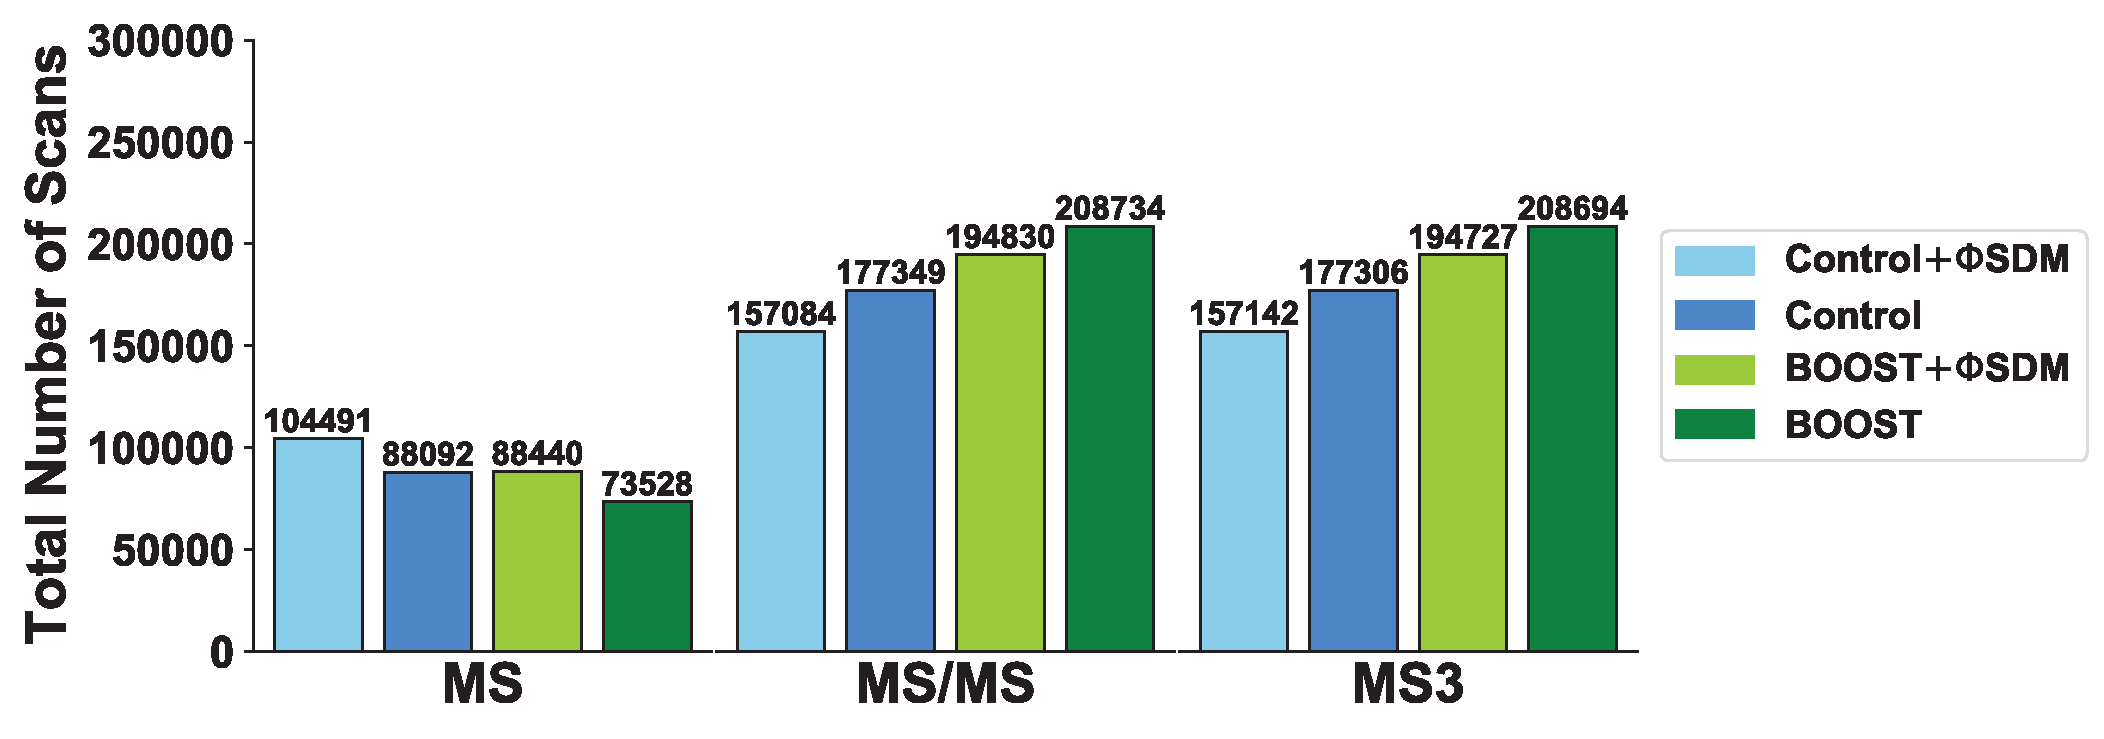
\includegraphics[width=175mm]{figures/supplements/scans.pdf}
%\caption{A bar chart showing the total number of MS, MS/MS and MS3 scans from each experiment. The numbers above each bar indicate the exact number of scans for that experiment. }\label{scans}
%\end{figure}

\clearpage

\begin{figure}[t!]
\centering
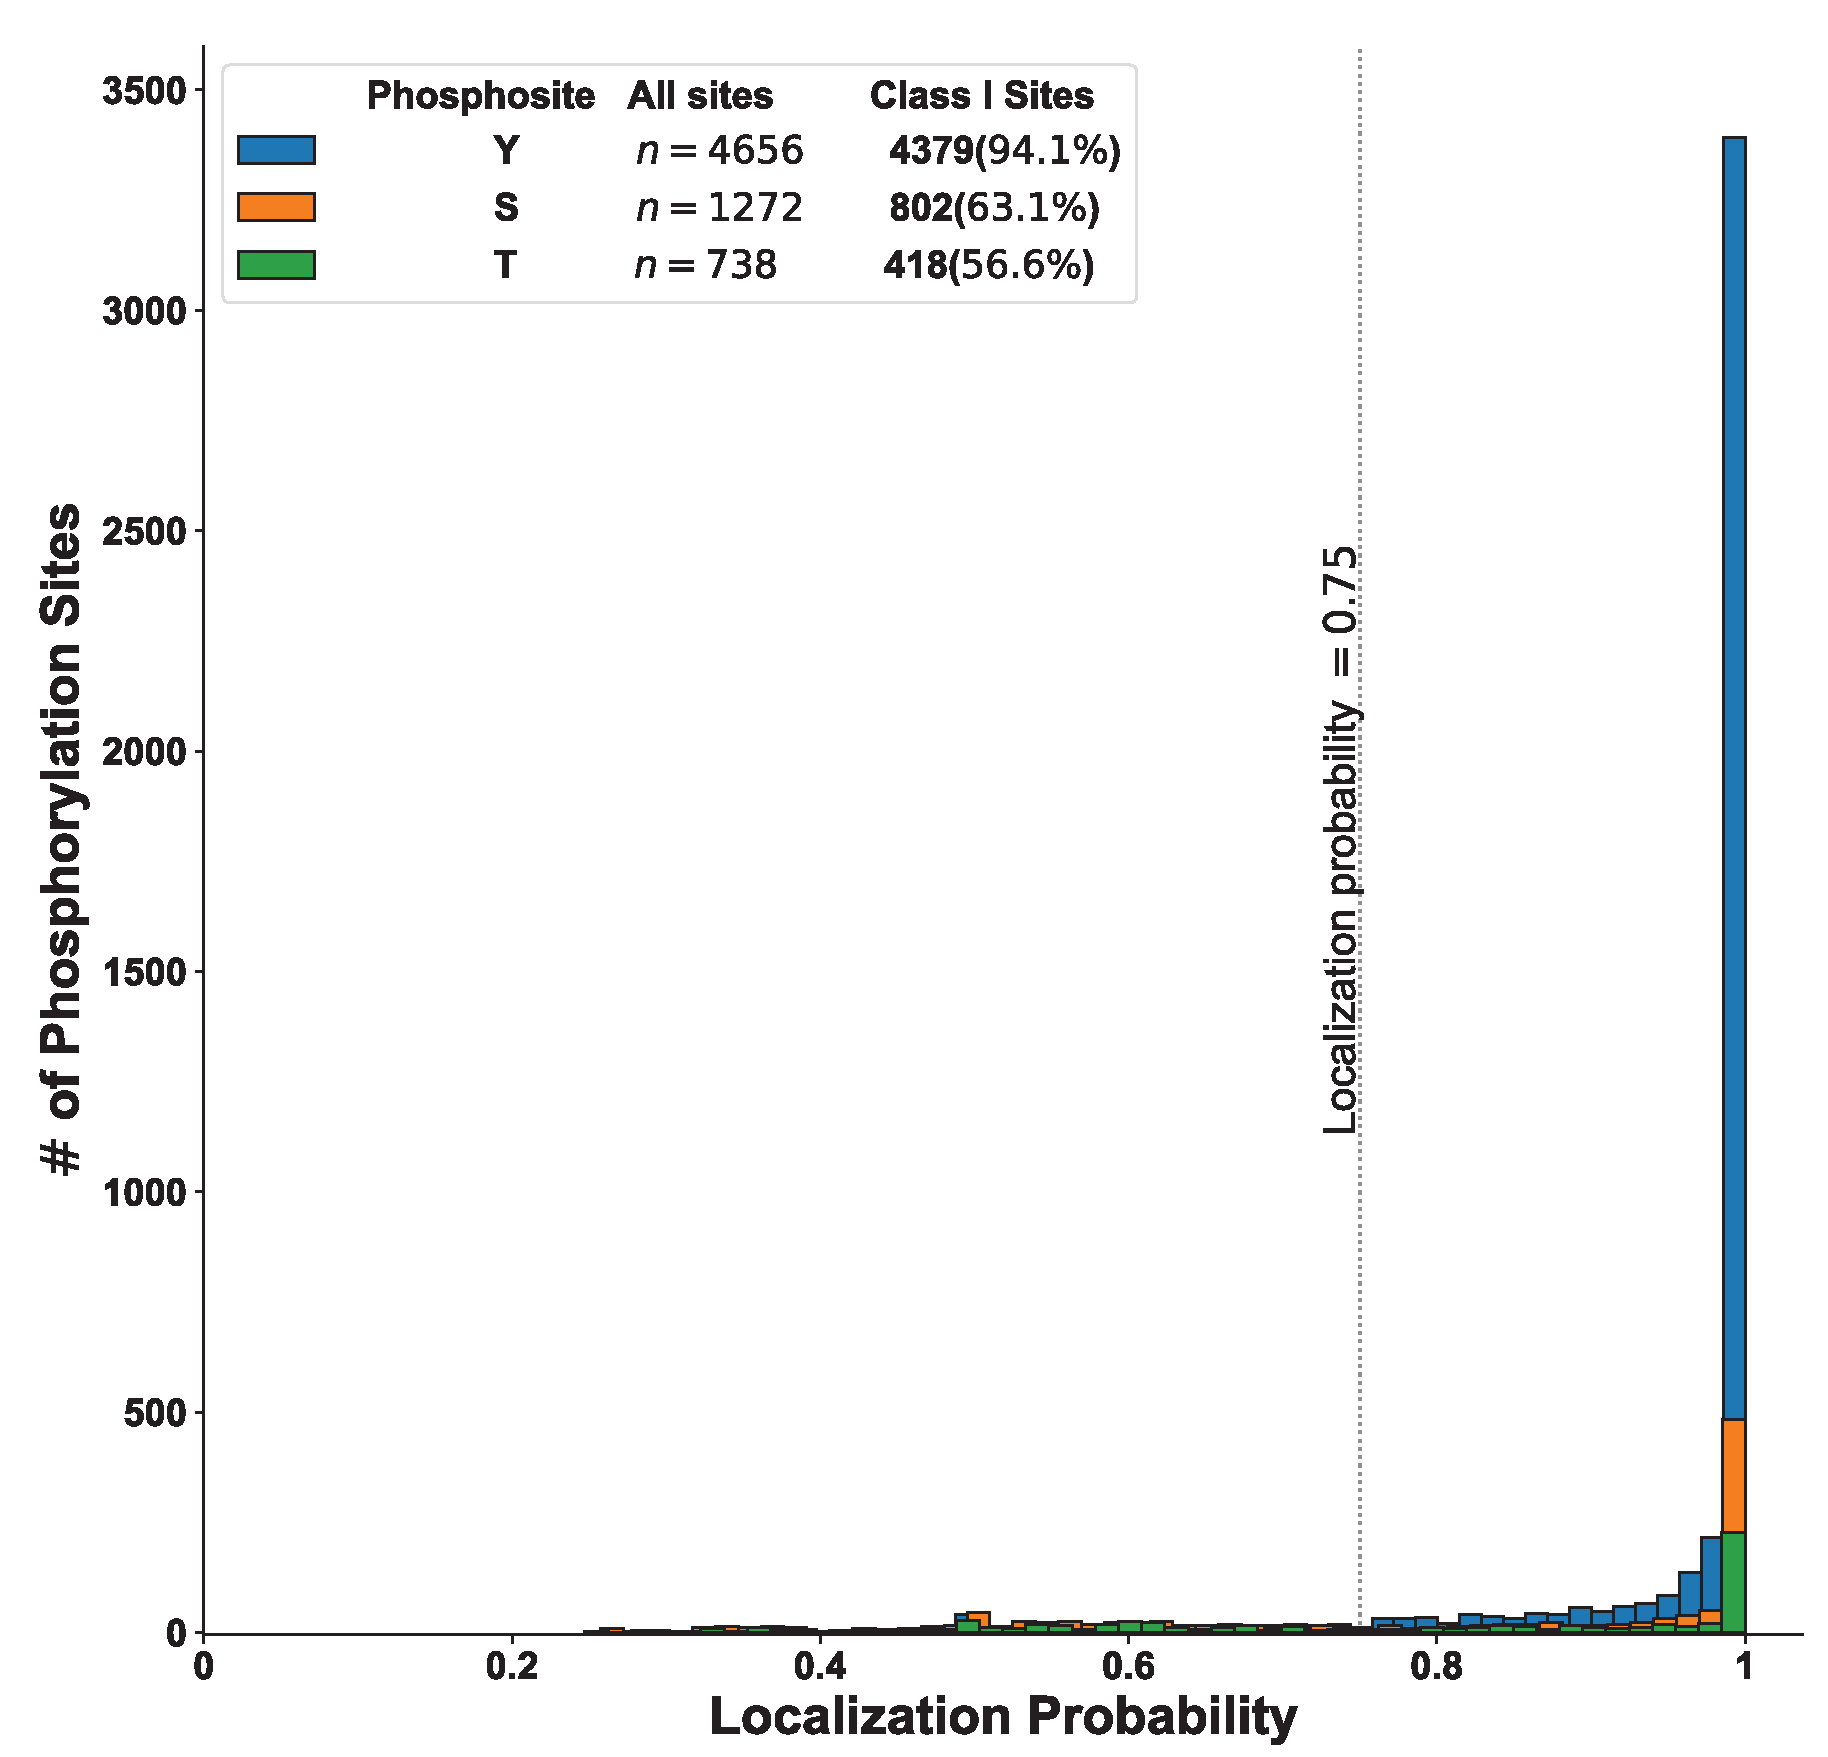
\includegraphics[width=175mm]{figures/supplements/locprob.pdf}
\caption{A histogram with depicting all PSMs from all experiments containing at least one phosphorylated serine (S), threonine (T), or tyrosine (Y) amino acid as a function of localization probability ($n_{\text{bins}} = 75$). The total number and number of Class I (localization probability $>0.75$) phosphorylation sites for each amino acid are noted in the Figure Legend.}\label{locprob}
\end{figure}


\begin{figure}
\centering
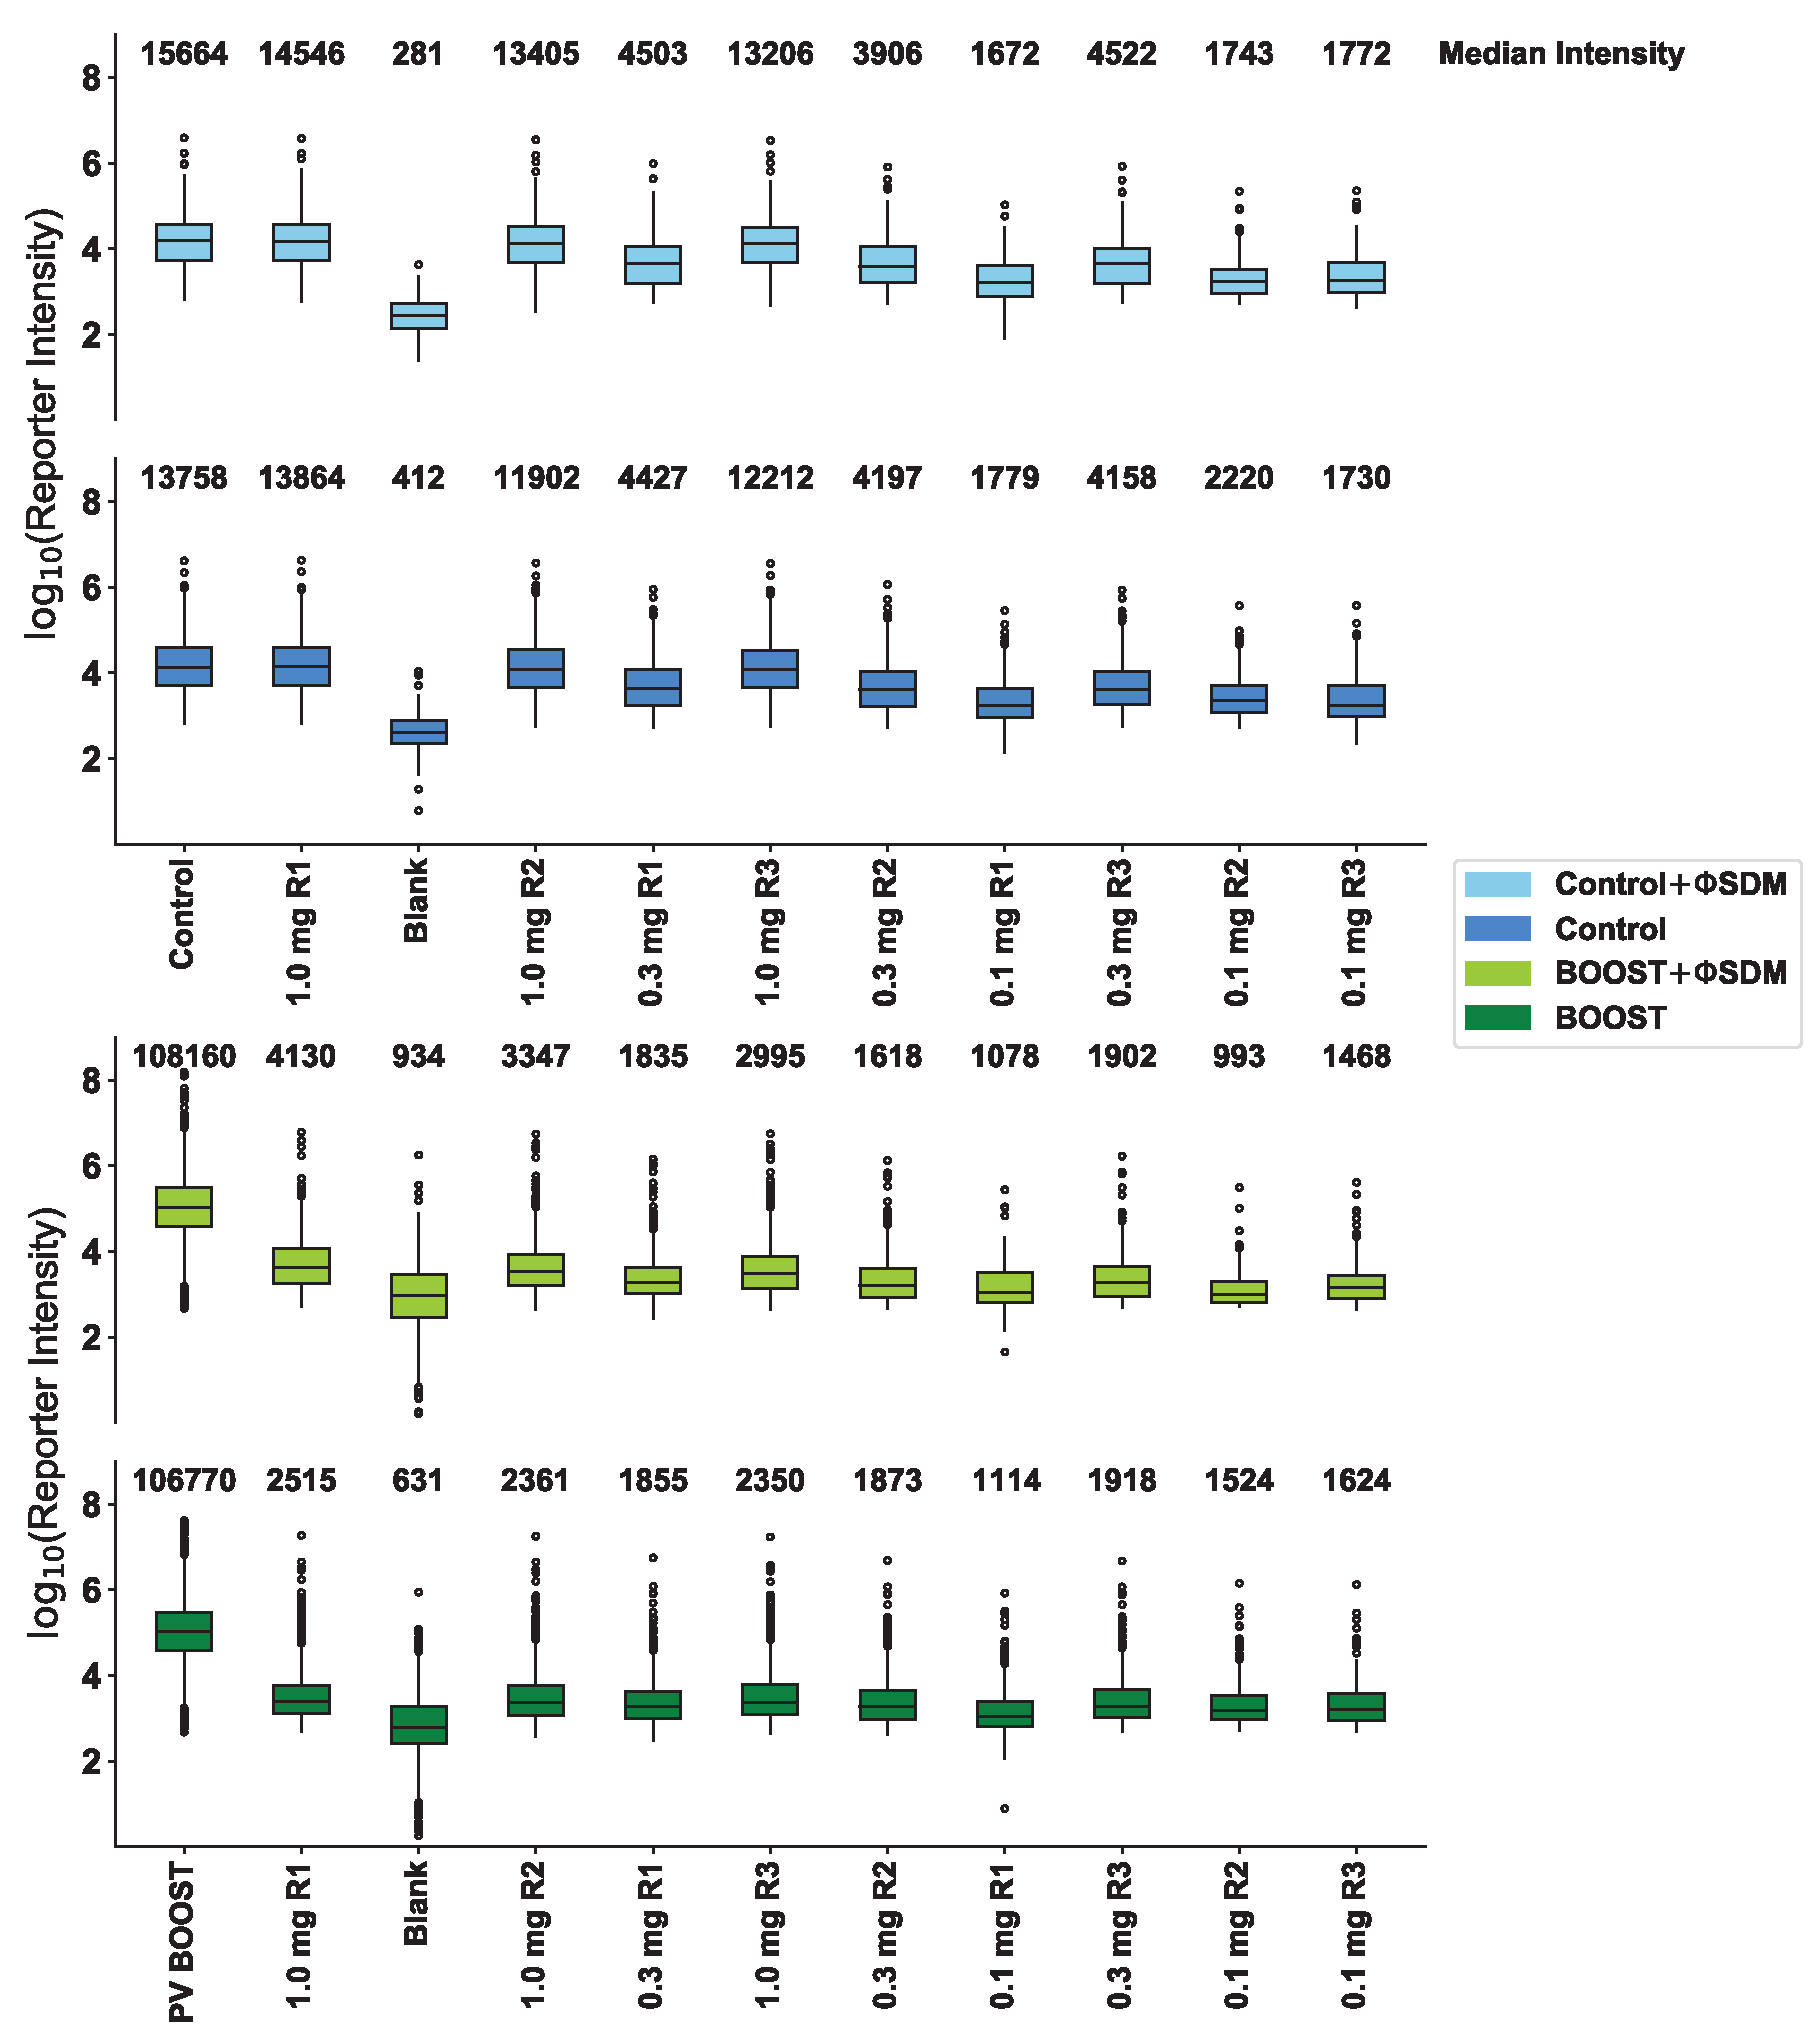
\includegraphics[width=150mm]{figures/supplements/intensity_plots.pdf}
\caption{Box-and-whisker plots showing the $\log_{10}$ transformed reporter intensities for each TMT mix and each condition. Non-transformed, median intensities are displayed above each box-and-whisker plot.}\label{intensity_plots}
\end{figure}

\clearpage

\begin{figure}[!t]
\centering
\includegraphics[width=175mm]{figures/supplements/boost_replicate_reprod.pdf}
\caption{Replicate reproducibility is stable when $\Phi$SDM is disabled for low protein input camples in the pervanadate BOOST condition. Evaluation of replicate reproducibility in the BOOST experiment (with $\Phi$SDM disabled) using pairwise comparisons of $\log_2$ transformed abundances for phosphopeptides with the same charge state and assigned sequence. For each comparison, we show the line of best fit as determined by simple least-squares regression, the $r^2$ value as an estimate of the quality of the fitted line, and the total number of points ($n$) in each comparison.}\label{boost_replicate_reprod}
\end{figure}

\clearpage

\begin{figure}[t!]
\centering
\includegraphics[width=175mm]{figures/supplements/boostsdm_replicate_reprod}
\caption{Replicate reproducibility is severely degraded when $\Phi$SDM is enabled for low protein input samples in the pervanadate BOOST condition. Evaluation of replicate reproducibility in the BOOST experiment (with $\Phi$SDM enabled) using pairwise comparisons of $\log_2$ transformed abundances for phosphopeptides with the same charge state and assigned sequence. For each comparison, we show the line of best fit as determined by simple least-squares regression, the $r^2$ value as an estimate of the quality of the fitted line, and the total number of points ($n$) in each comparison. }\label{boostsdm_replicate_reprod}
\end{figure}

\clearpage

\begin{figure}[t!]
\centering
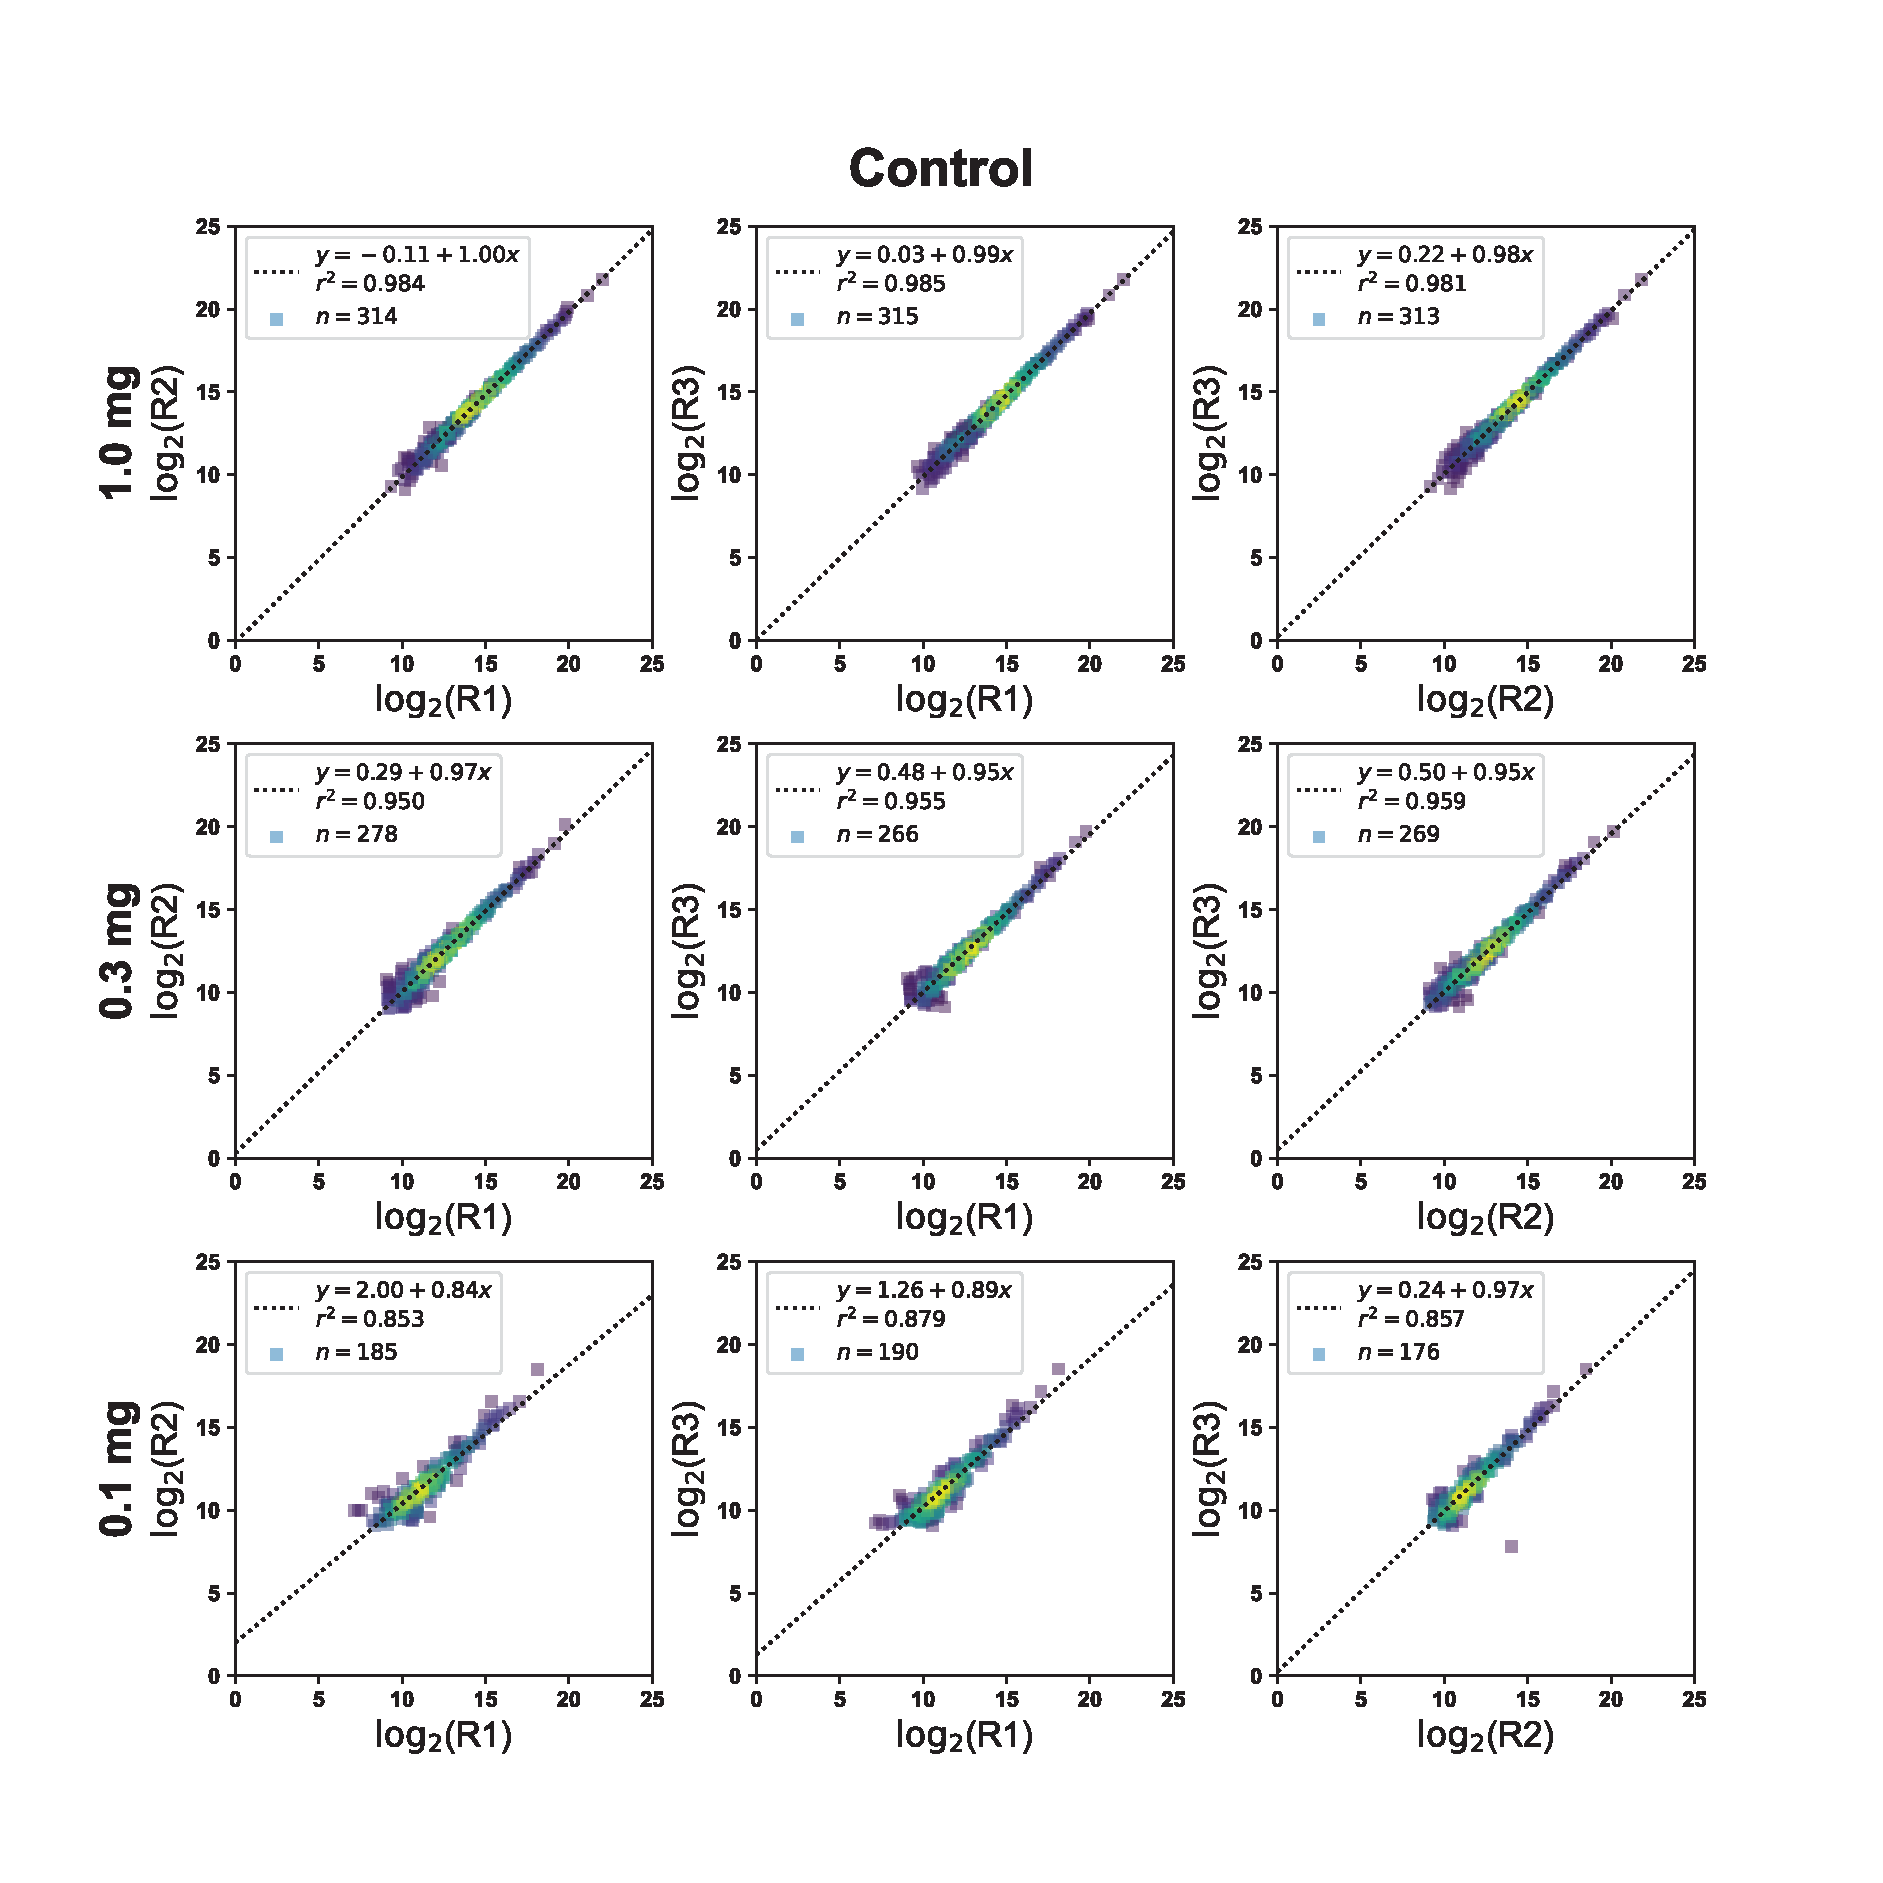
\includegraphics[width=175mm]{figures/supplements/control_replicate_reprod.pdf}
\caption{Replicate reproducibility is stable when $\Phi$SDM is disabled for low protein input camples in the $1.0$ mg Control condition. Evaluation of replicate reproducibility in the $1.0$ mg Control experiment (with $\Phi$SDM disabled) using pairwise comparisons of $\log_2$ transformed abundances for phosphopeptides with the same charge state and assigned sequence. For each comparison, we show the line of best fit as determined by simple least-squares regression, the $r^2$ value as an estimate of the quality of the fitted line, and the total number of points ($n$) in each comparison. }\label{control_replicate_reprod}
\end{figure}

\clearpage

\begin{figure}[t!]
\centering
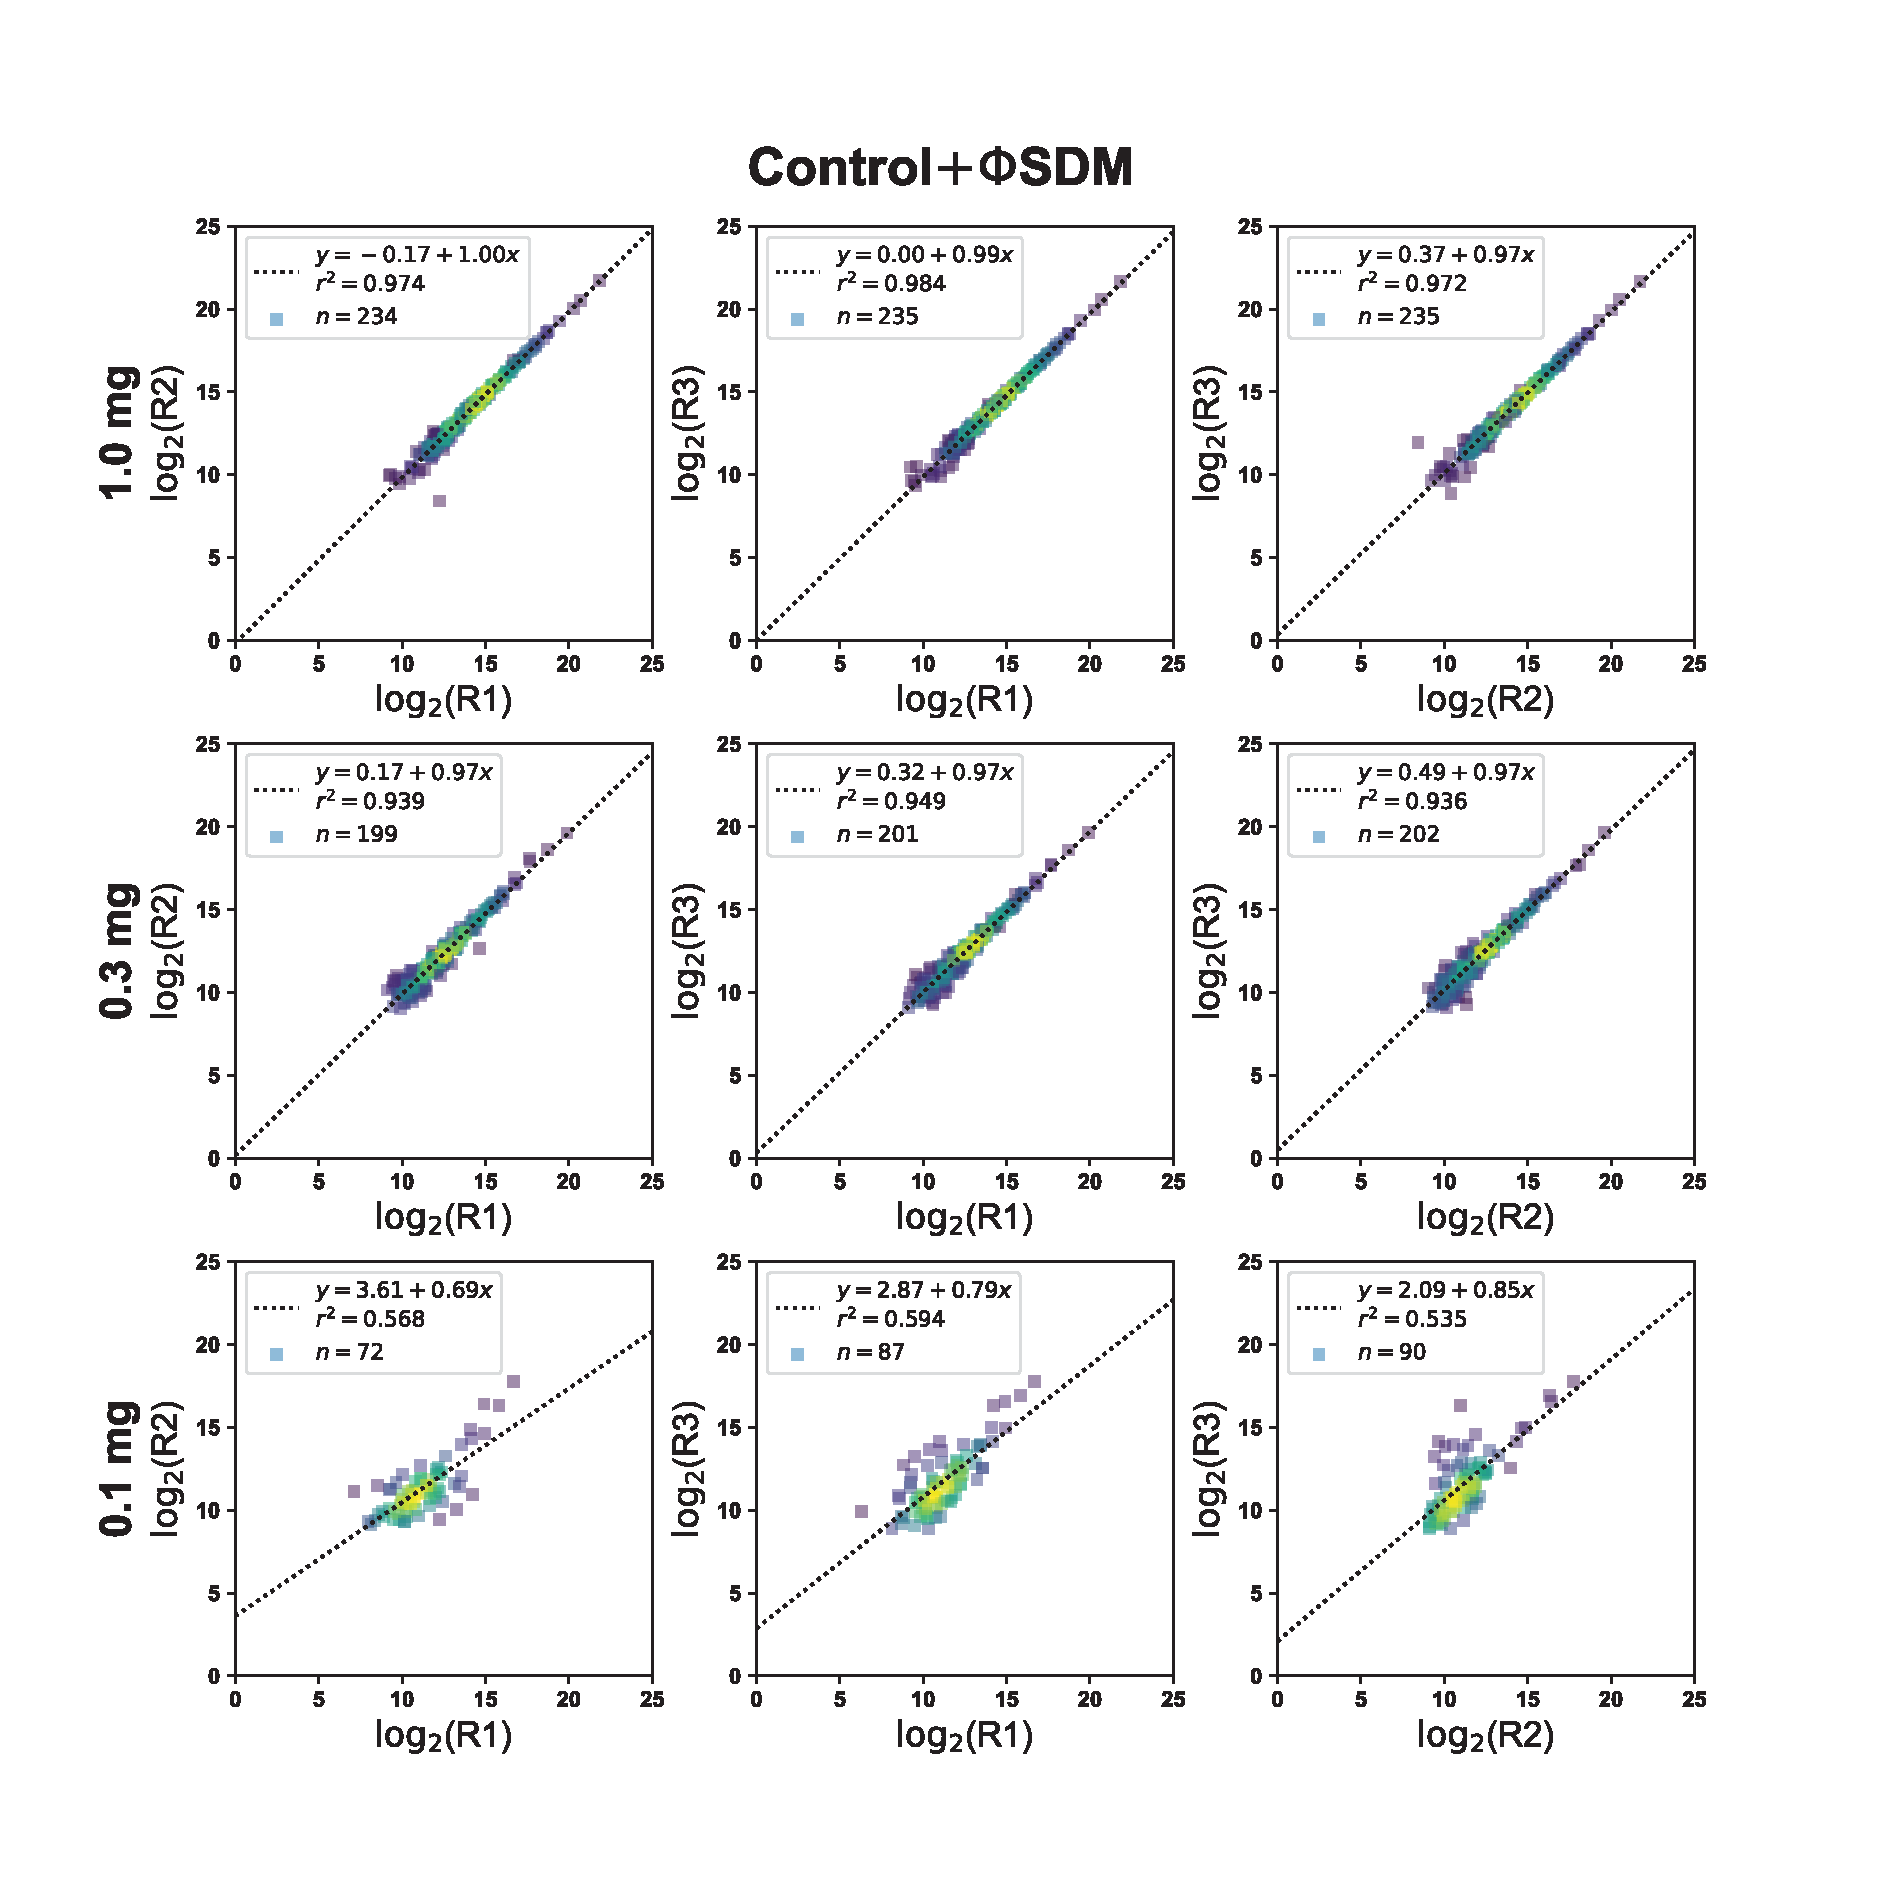
\includegraphics[width=175mm]{figures/supplements/controlsdm_replicate_reprod.pdf}
\caption{Replicate reproducibility is degraded when $\Phi$SDM is enabled for low protein input samples in the $1.0$ mg Contro conditionl. Evaluation of replicate reproducibility in the $1.0$ mg experiment (with $\Phi$SDM enabled) using pairwise comparisons of $\log_2$ transformed abundances for phosphopeptides with the same charge state and assigned sequence. For each comparison, we show the line of best fit as determined by simple least-squares regression, the $r^2$ value as an estimate of the quality of the fitted line, and the total number of points ($n$) in each comparison. }\label{controlsdm_replicate_reprod}
\end{figure}

\clearpage

\begin{figure}[t!]
\centering
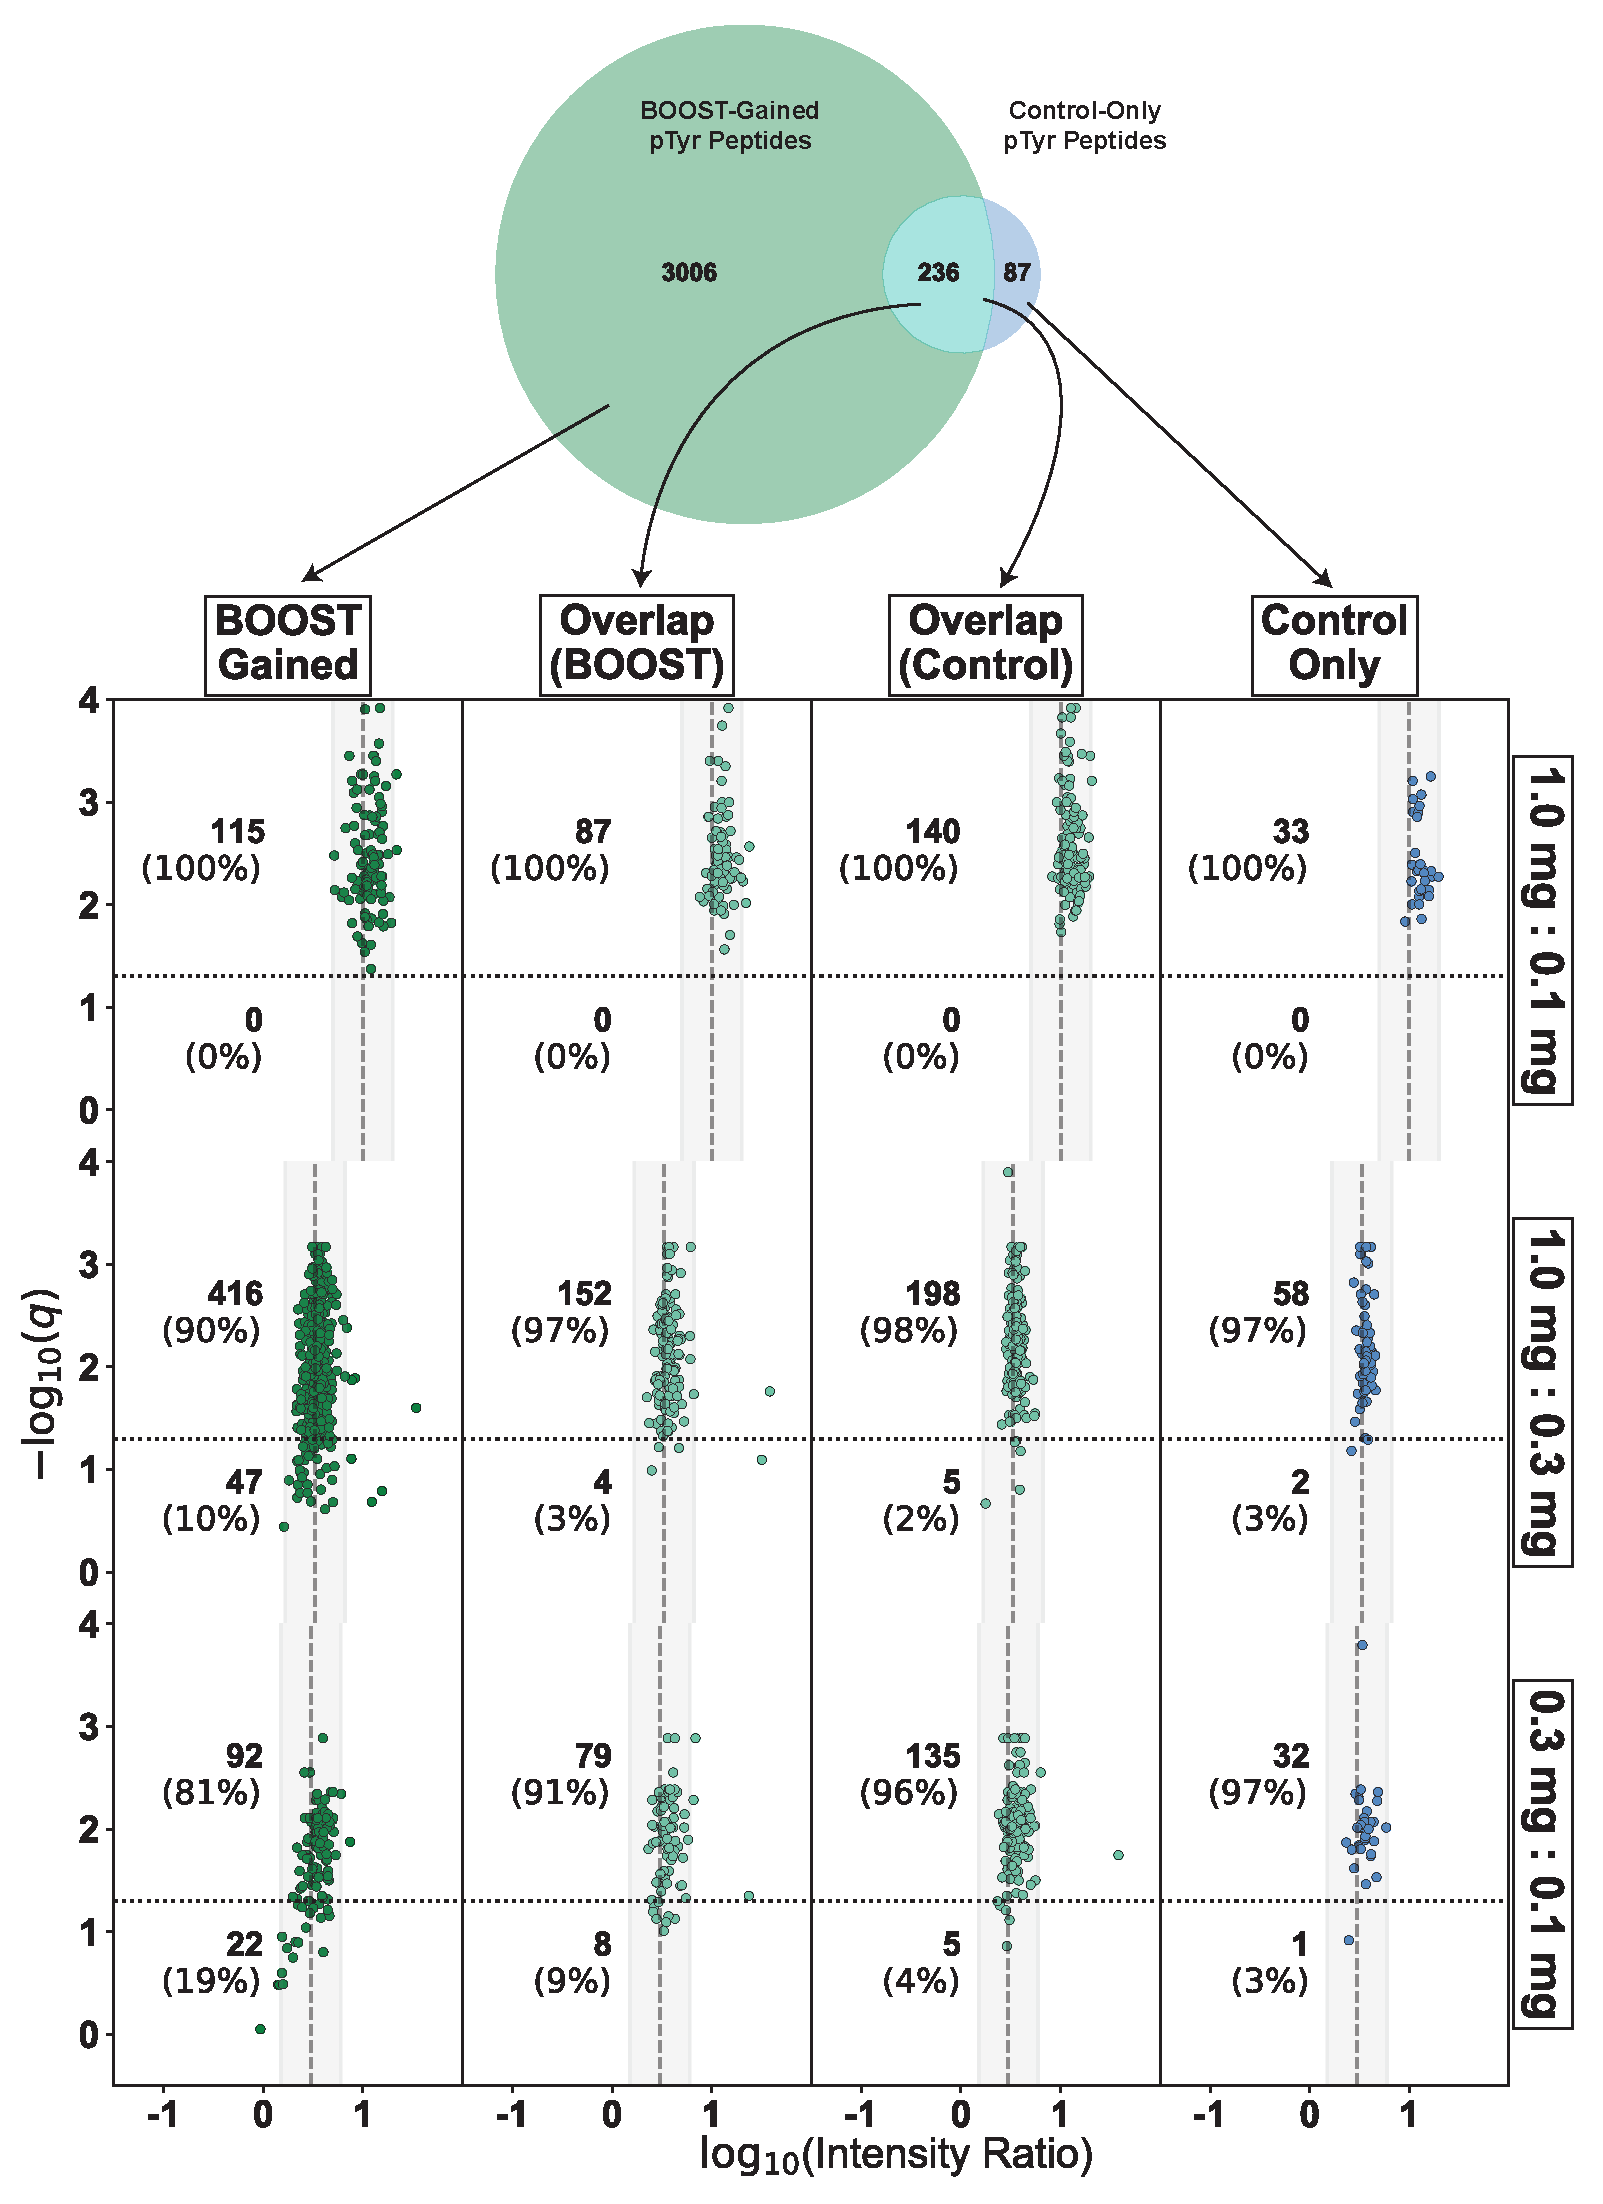
\includegraphics[width=135mm]{figures/supplements/boost_control_gained_qvolcanoes.pdf}
\caption{With $\Phi$SDM disabled, the pervanadate BOOST channel dramatically increases the number of unique pTyr peptides observed as compared to a $1.0$ mg Control channel. A Venn diagram showing the overlap of unique pTyr peptides between the BOOST and $1.0$ mg Control experiments (with $\Phi$SDM disabled). Volcano plots show $-\log_{10}(q\text{-value})$ as a function of $\log_{10}(\text{Intensity Ratio})$ for unique pTyr peptides from groups show in the Venn diagram. For the overlapping section, volcano plots were created using data from both the BOOST experiment and the control experiment acquired with $\Phi$SDM disabled. }\label{boost_control_gained_qvolcanoes}
\end{figure}


%\addtocounter{figure}{-1}
%\begin{figure}[t!]
%\caption{With $\Phi$SDM disabled, the pervanadate BOOST channel dramatically increases the number of unique pTyr peptides observed as compared to a $1.0$ mg Control channel. A Venn diagram showing the overlap of unique pTyr peptides between the BOOST and $1.0$ mg Control experiments (with $\Phi$SDM disabled). Volcano plots show $-\log_{10}(q\text{-value})$ as a function of $\log_{10}(\text{Intensity Ratio})$ for unique pTyr peptides from the BOOST experiment only (``BOOST Gained"), BOOST and Control overlap (from the BOOST experiment; ``BOOST $\cap$ Control"), Control and BOOST overlap (from the Control experiment; ``Control $\cap$ BOOST"), and Control experiment only (``Control Only"). }\label{boost_control_gained_qvolcanoes}
%\end{figure}

\clearpage

\begin{figure}[t!]
\centering
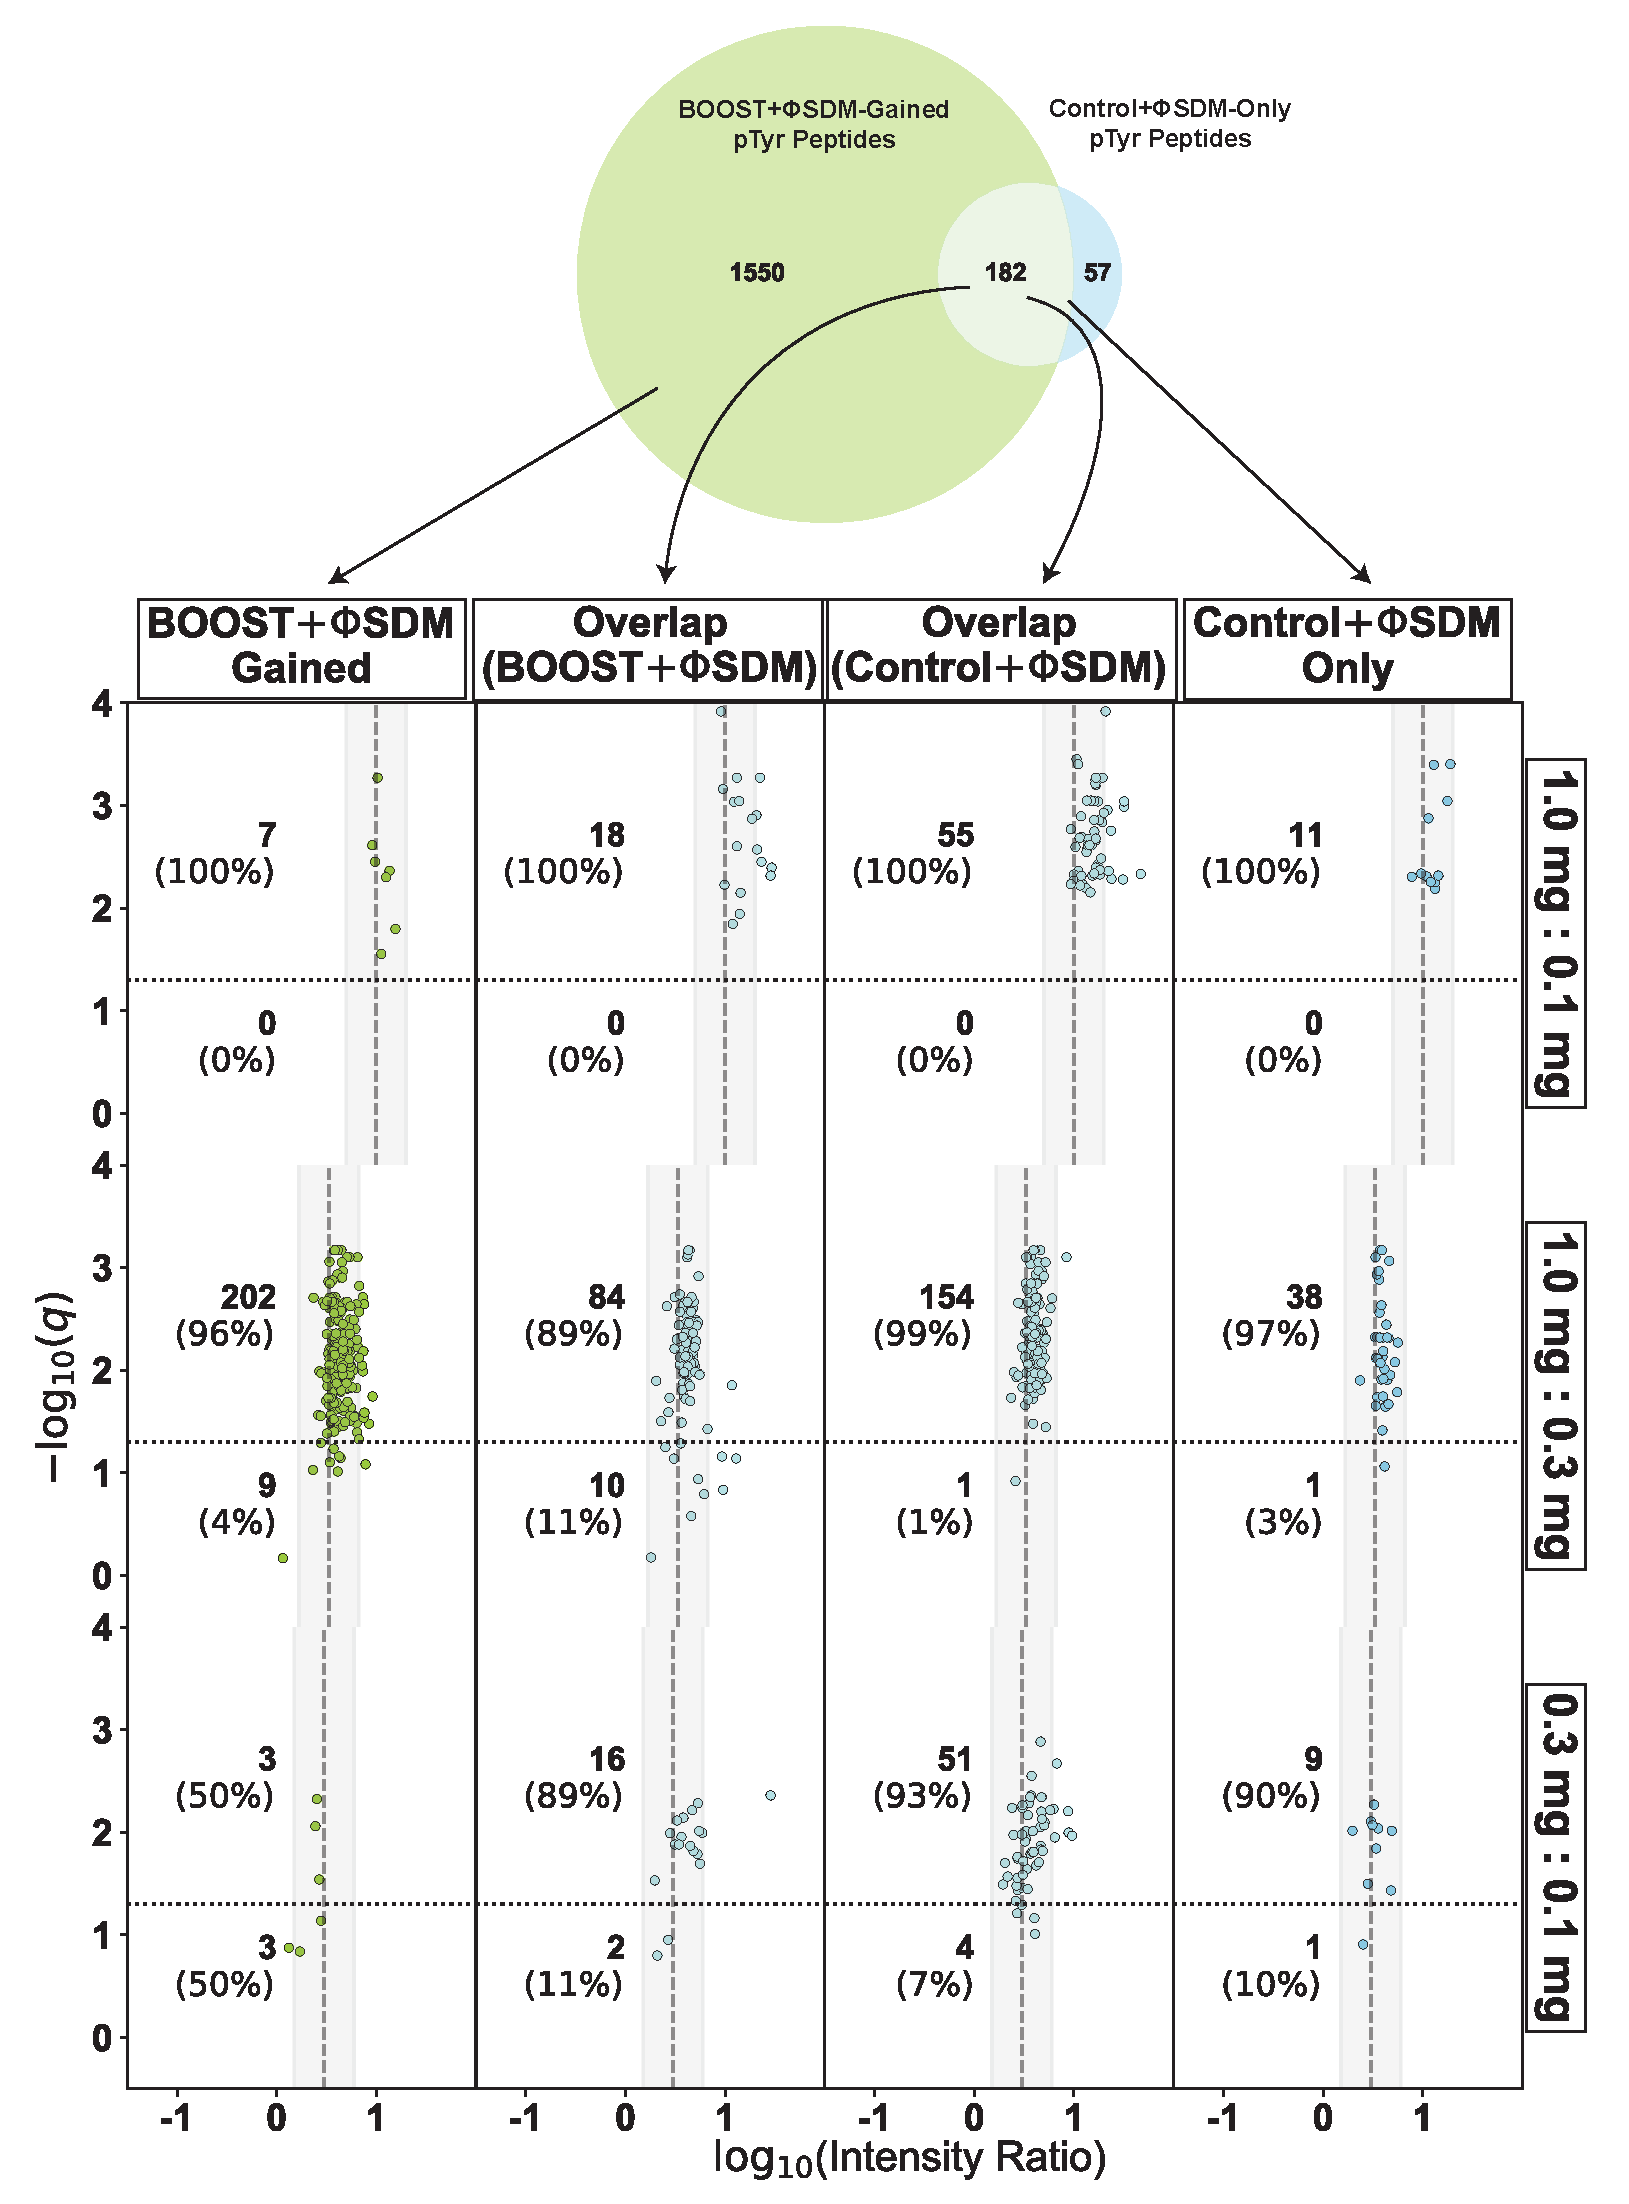
\includegraphics[width=135mm]{figures/supplements/boostsdm_controlsdm_gained_qvolcanoes.pdf}
\caption{The pervanadate BOOST channel increases the number of unique pTyr peptides observed when $\Phi$SDM is enabled, although few peptides are observed in low abundance samples. A Venn diagram showing the overlap of unique pTyr peptides between the BOOST$+\Phi$SDM and $1.0$ mg Contro$+\Phi$SDMl experiments. Volcano plots show $-\log_{10}(q\text{-value})$ as a function of $\log_{10}(\text{Intensity Ratio})$ for unique pTyr peptides from groups show in the Venn diagram. For the overlapping section, volcano plots were created using data from both the BOOST experiment and the control experiment acquired with $\Phi$SDM enabled. }\label{boostsdm_controlsdm_gained_qvolcanoes}
\end{figure}

%\addtocounter{figure}{-1}
%\begin{figure}[t!]
%\caption{The pervanadate BOOST channel increases the number of unique pTyr peptides observed when $\Phi$SDM is enabled, although few peptides are observed in low abundance samples. A Venn diagram showing the overlap of unique pTyr peptides between the BOOST$+\Phi$SDM and $1.0$ mg Contro$+\Phi$SDMl experiments. Volcano plots show $-\log_{10}(q\text{-value})$ as a function of $\log_{10}(\text{Intensity Ratio})$ for unique pTyr peptides from the BOOST$+\Phi$SDM experiment only (``BOOST$+\Phi$SDM Gained"), BOOST$+\Phi$SDM and Control$+\Phi$SDM overlap (from the BOOST$+\Phi$SDM experiment; ``BOOST$+\Phi$SDM $\cap$ Contro$+\Phi$SDMl"), Contro$+\Phi$SDMl and BOOST$+\Phi$SDM overlap (from the Control$+\Phi$SDM experiment; ``Control$+\Phi$SDM $\cap$ BOOST$+\Phi$SDM"), and Control$+\Phi$SDM experiment only (``Control$+\Phi$SDM Only"). }\label{boostsdm_controlsdm_gained_qvolcanoes}
%\vspace*{5cm}
%\end{figure}

\clearpage

\begin{figure}[t!]
\centering
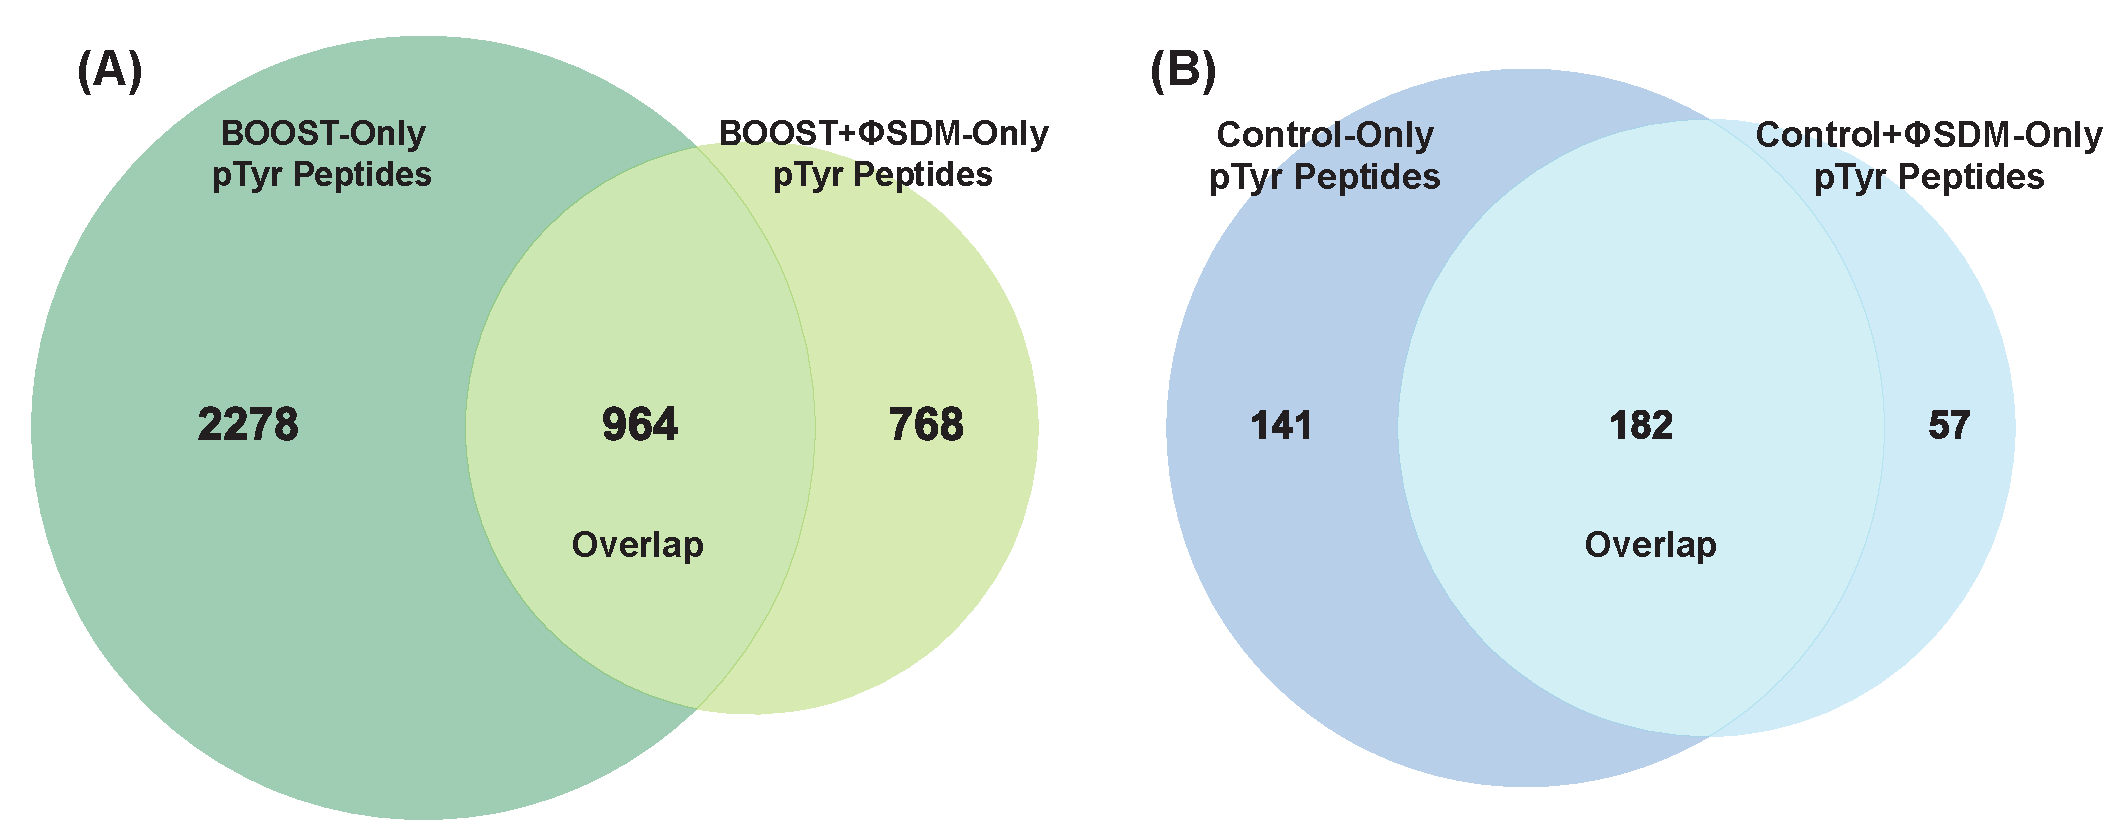
\includegraphics[width=165mm]{figures/supplements/set_overlap_2.pdf}
\caption{Enabling $\Phi$SDM results in lower yield in both pervanadate BOOST and $1.0$ mg Control conditions. Venn diagrams showing the number of unique pTyr peptides observed when $\Phi$SDM is enabled or disabled using (A) pervanadate BOOST samples, and (B) $1.0$ mg Control samples.}\label{set_overlap_2}
\end{figure}

\clearpage

\begin{figure}[t!]
\centering
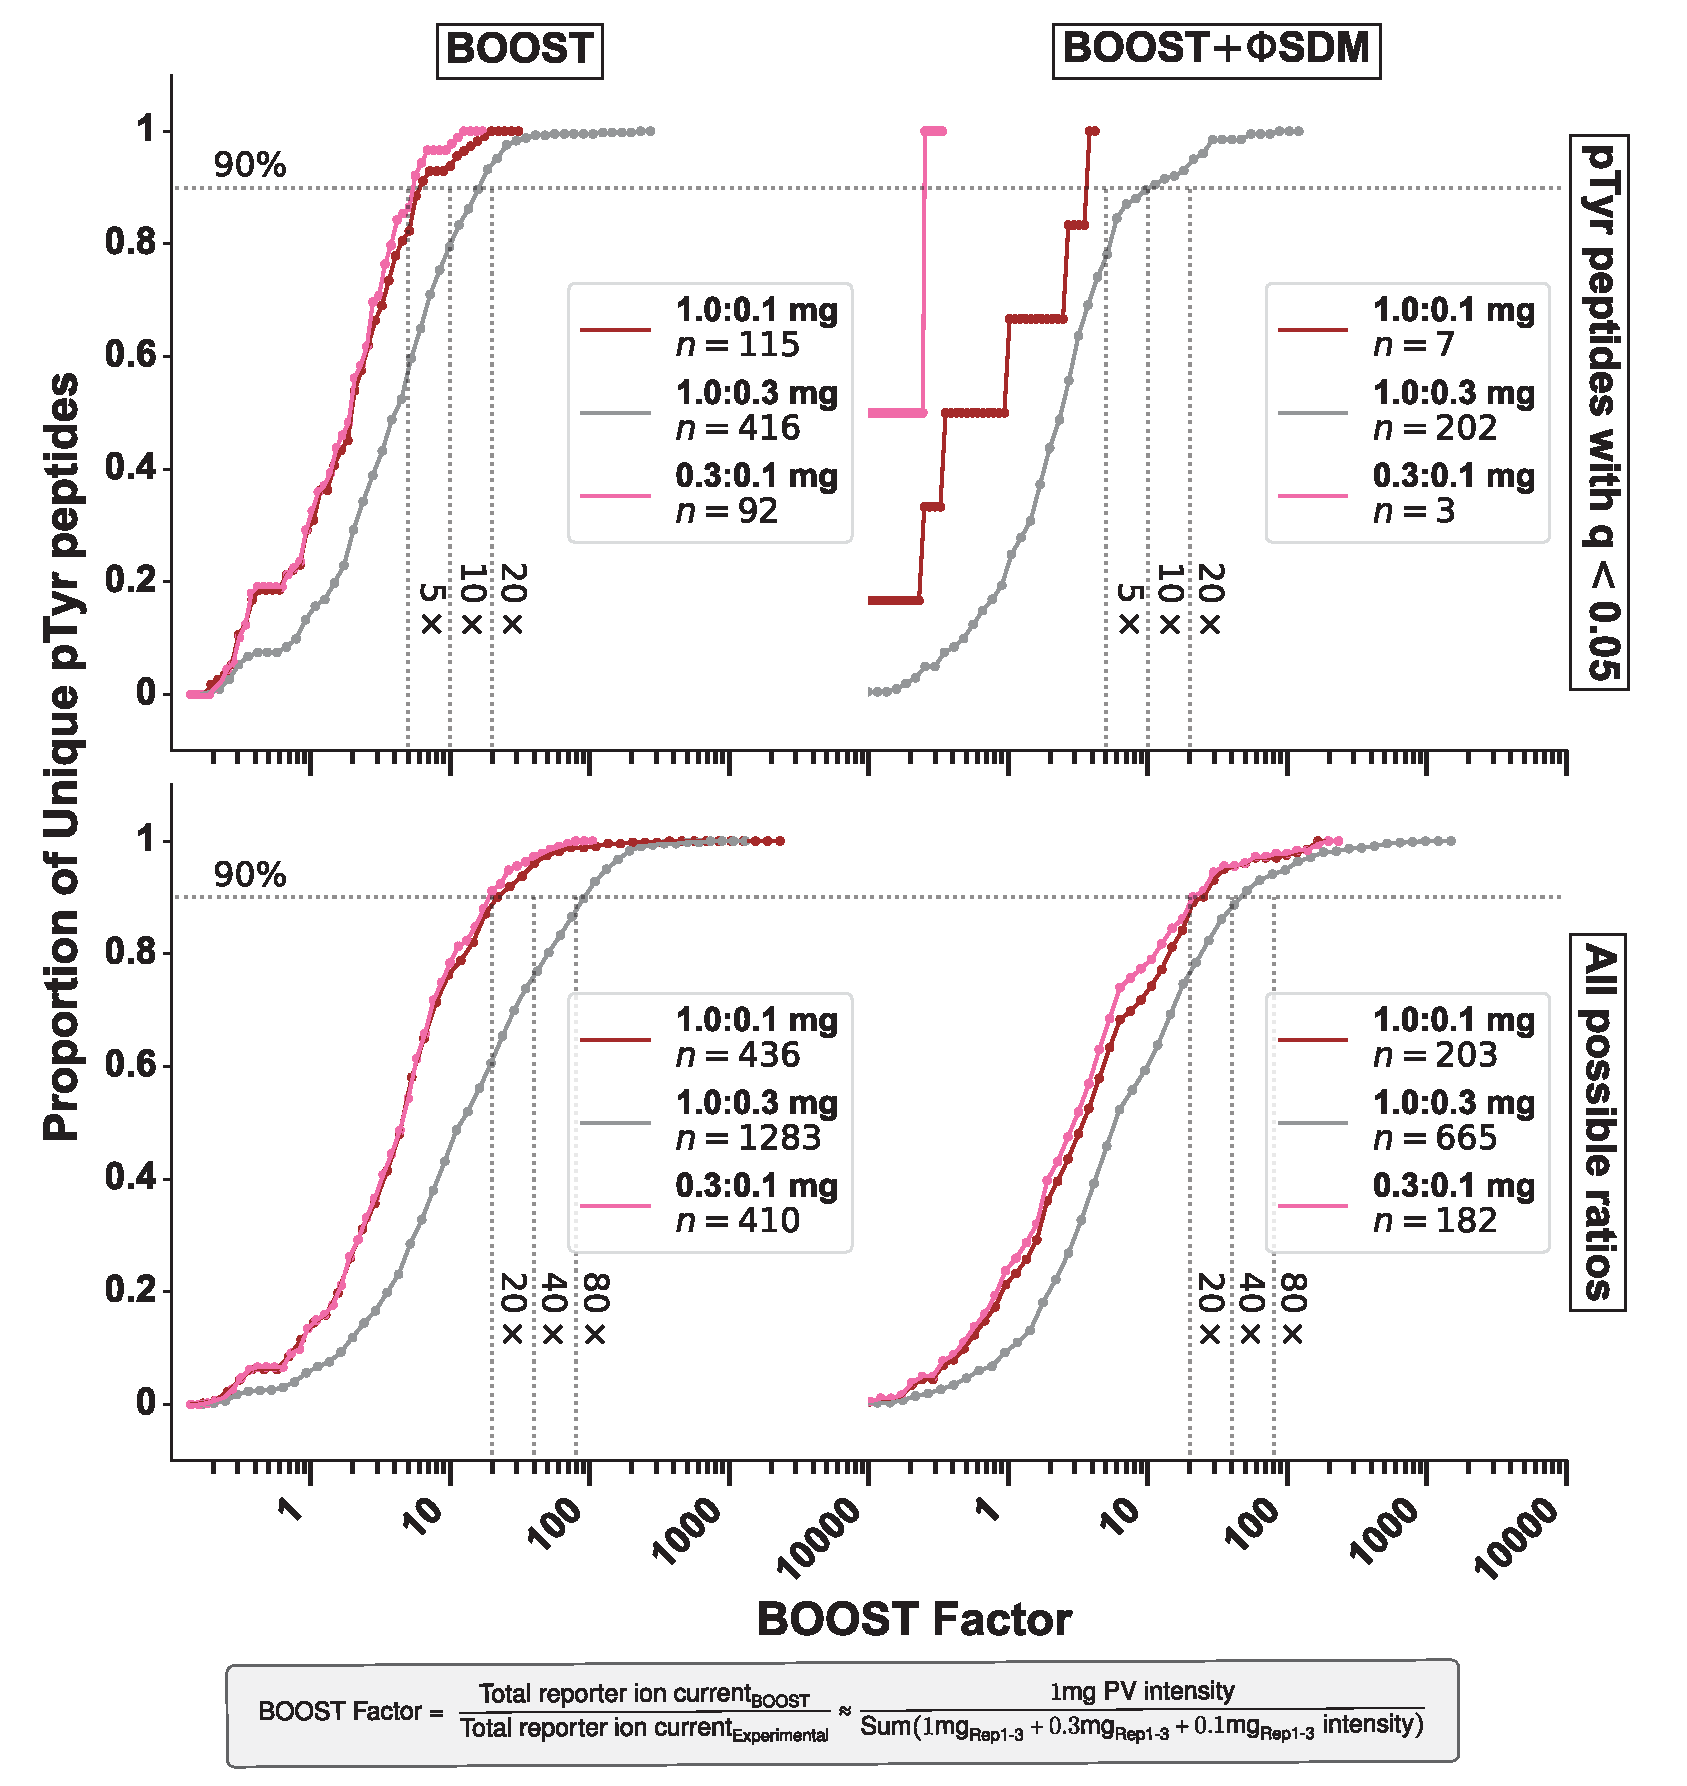
\includegraphics[width=165mm]{figures/supplements/boost_factor_cdfs.pdf}
\caption{Enabling $\Phi$SDM decreases quantitation depth, particularly in low abundance samples. Cumulative distribution of BOOST factors for unique pTyr peptides identified in the pervanadate BOOST experiments with $\Phi$SDM disabled or with $\Phi$SDM enabled for pTyr peptides with a statistically significant ratio ($q<0.05$) or for all calculable ratios. For each cumulative distribution, the range of BOOST factors are split into $50$ bins of equal size on a $\log_{10}$ scale. }\label{boost_factor_cdfs}
\end{figure}

\end{document}




























